\section{fork.c}

	Muestre la pantalla de ejecucución del programa:

	\begin{center}
		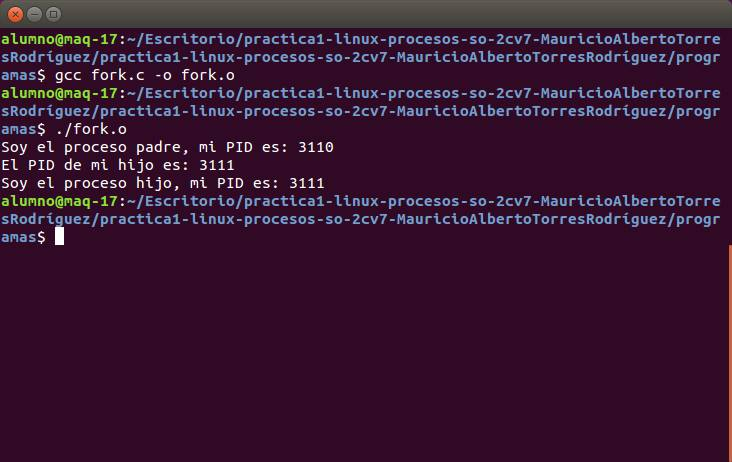
\includegraphics[width=\linewidth]{imagenes/forkc.png}
	\end{center}

	Para las siguientes funciones, mencione dónde están definidas, cúal es su propósito, qué es lo que proporcionan de salida y qué argumentos necesitan de entrada:

	\begin{itemize}

		\item perror (print error)
		\\ Esta funcion se encarga de al recibir una señal de error, este se encarga de mapearlo(un valor, que convierte posteriormente en secuencia de caracteres, para crear un mensaje) lo imprime en el stream de error, seguido por dos puntos y un espacio. (si cadena no es un puntero nulo y el carácter apuntado por cadena no es el carácter nulo), la cadena apuntada por cadena seguido de dos puntos y un espacio 
		\\Esta funcion se encuentra dentro de la libreria <stdio.h>, y recibe los valores de apuntador a una cadena, y regresa un valor tipo void.
		\item fork
		\\Esta funcion nos permite crear procesos al igual que la funcion clone, pero en el caso de fork, ésta nos permite crear un proceso hijo con lo mismos valores que el padre, a excepcion de el ID del proceso, y de el espacio de memoria que está ocupando, aún así, si los valores de alguno de los dos se modifican, el otro conserva los valores de sus variables, sin verse afectado por el otro. De parte del task\_struct del padre se copian los campos, y esos son asignados al hijo, pero con otro identificador, posteriormente, el hijo hace una llamada al sistema con la funcion exec.
		\\Esta funcion se encuentra en la libreria <unistd.h> y recibe los valores de el PID (numero identificador del proceso) y regresa una nueva direccion donde se creará al proceso hijo con los mismos valores, a excepcion del PID. 

	\end{itemize}

	Responda lo siguiente:

	\begin{itemize}

		\item ¿Qué pasa cuando la varible hijo tiene un valor de 0 (cero)? Significa que el proceso que tiene esa variable es el hijo.
		\item ¿Qué pasa cuando la variable hijo tiene un valor mayor que 0 (cero)? Significa que el proceso que tiene esa variable es el padre.
		\item Suponga que la variable hijo es mayor que 0 (cero), ¿qué representa dicho número? El ID del proceso hijo.

	\end{itemize}
	